\section{Validation}
\label{sec:validation}

\subsection{Lid-driven cavity (pure fluid)}
The centreline velocity $u(y)$ at $x=0.5$ is compared to Ghia \emph{et al.}
\cite{Ghia1982}. The MAC solver attains an RMS error of $1.7\times10^{-3}$ at
$\mathrm{Re}=100$ and $2.8\times10^{-2}$ at $\mathrm{Re}=1000$ ($N=129$). The implicit
(IMEX) integrator reproduces the same steady state (RMS $1.68\times10^{-2}$ vs.\
explicit $1.71\times10^{-2}$ at $N=48$) and remains correct at $5\times$ the explicit
viscous CFL. \TODO{final high-resolution Ghia figure/table.}

\subsection{Soft disc in a lid-driven cavity (FSI)}
A neo-Hookean disc carried by the cavity flow is compared to the full-Eulerian result of
Sugiyama \emph{et al.}\ \cite{Sugiyama2011} and to Jain \emph{et al.}\ \cite{Jain2019}.
The centroid trajectory matches the reference and the deformed interface is
grid-converged ($N=64\approx N=128$). The IMEX integrator reproduces the explicit
(validated) centroid trajectory to $2\times10^{-3}$ with identical minimum Jacobian,
confirming that the implicit viscosity does not perturb the validated FSI result
(\cref{fig:disc-centroid}, \cref{tab:disc-integrators}). Over the full inward spiral the
explicit, IMEX and monolithic integrators trace the same centroid path---with the
monolithic completing it in a quarter of the steps (\cref{sec:disc-speedup}).

\begin{figure}[t]\centering
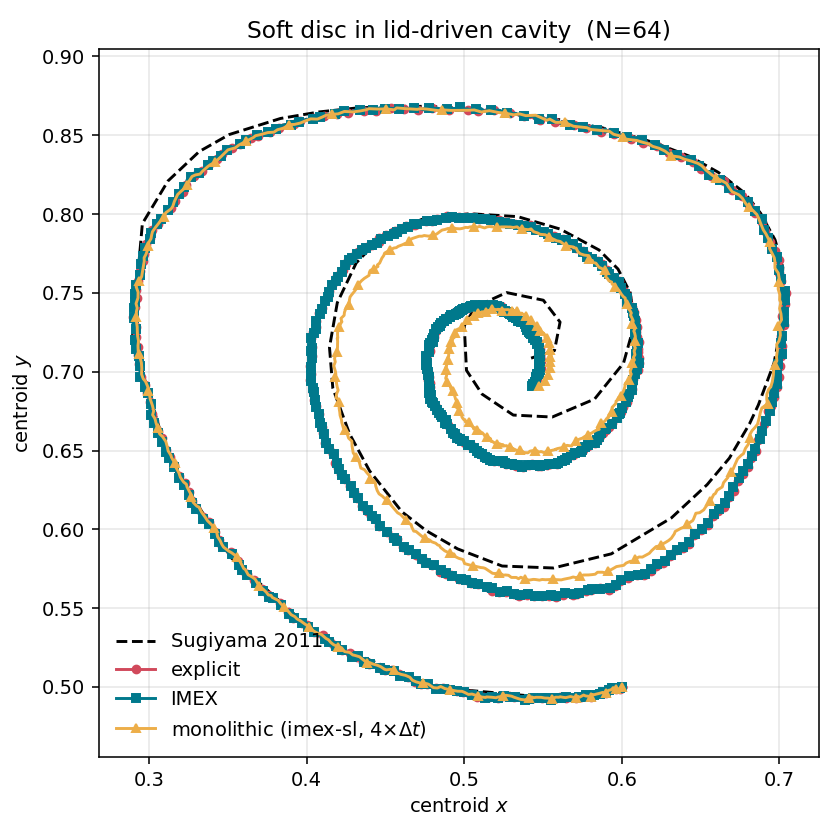
\includegraphics[width=0.62\linewidth]{figures/soft_disc_overlay.png}
\caption{Soft disc in a lid-driven cavity ($N{=}64$): centroid trajectory over the full
inward spiral for the explicit, IMEX and monolithic integrators, compared with Sugiyama
\emph{et al.}\ \cite{Sugiyama2011}. Explicit and IMEX are indistinguishable; the
monolithic (semi-Lagrangian, $4\times\dt$) traces the same spiral in ${\sim}4\times$ fewer
steps, with a small phase drift on the innermost turns.}
\label{fig:disc-centroid}
\end{figure}

\subsection{Soft disc in a Taylor--Green vortex (energy)}
The kinetic and strain energies exchange periodically while the total energy is
conserved; the spatial convergence of the energies is second order, with velocity and
pressure limited to first order by the diffuse interface. \TODO{energy-exchange figure
and convergence table.}

\subsection{Surface tension}
The static Laplace jump $\Delta p=\gamma/R$ is captured to $0.4\%$ with bounded parasitic
currents (balanced-force CSF). \TODO{oscillating-drop Lamb-frequency dynamic test.}
